\documentclass[]{article}
\usepackage{geometry}   % my added package "geometry"
\geometry{letterpaper,tmargin=1in,bmargin=1in,lmargin=2.2cm,rmargin=2.2cm}
\usepackage[colorlinks,bookmarksopen,bookmarksnumbered,
citecolor=green,urlcolor=red]{hyperref}
\hypersetup{pdfauthor={Name}}
%%%%%%%%%%%%%%%%%%%%%%%%%%%%%%%%%%%%%%%%%%%%%%%%%%%%%%%%%%%%%%%%%%%%%%%%%
%\usepackage{graphicx}
\usepackage{graphics}
\usepackage{subcaption}
\usepackage{epsfig}
\usepackage{epstopdf}
\usepackage{amsfonts}
\usepackage{amssymb}
\usepackage{booktabs}
\usepackage{color,soul}
%%%%%%%%%%%%%%%%%%%%%%%%%%%%%%%%%%%%%%%%%%%%%%%%%%%%%%%%%%%%%%%%%
\usepackage{amsmath}
\usepackage{cleveref}
\usepackage{authblk}
%\usepackage[fleqn]{amsmath}
\usepackage{lineno}
\usepackage{tikz}
\usepackage{standalone}
\usetikzlibrary{calc,patterns,arrows.meta,shapes.arrows,intersections,positioning}
\usetikzlibrary{decorations.pathmorphing,backgrounds,fit,petri}
\usepackage[percent]{overpic}
%%%%%%%%%%%%%%%%%%%%%%%%%%%%%%%%%%%%%%%%%%%%%%%%%%%%%%%%%%%%%%%%%
\usepackage{xcolor}
\usepackage{listings}
\lstset { %
	language=C++,
	backgroundcolor=\color{blue!5}, % set backgroundcolor
	basicstyle=\footnotesize\color{black},% basic font settingbasicstyle=\ttfamily\color{black}
	keywordstyle=\color{red},
	commentstyle=\color{violet},
	stringstyle=\color{blue},
	xleftmargin=2em,
	frame=single,
	framexleftmargin=2em,
	numbers=left,
	numberstyle=\tiny,
	numbersep=8pt,
}
%%%%%%%%%%%%%%%%%%%%%%%%%%%%%%%%%%%%%%%%%%%%%%%%%%%%%%%%%%%%%%%%%
\renewcommand\thesubsection{\thesection\Alph{subsection}}
%%%%%%%%%%%%%%%%%%%%%%%%%%%%%%%%%%%%%%%%%%%%%%%%%%%%%%%%%%%%%%%%%
\renewcommand\lstlistingname{Header}
\renewcommand\lstlistlistingname{Header}
%%%%%%%%%%%%%%%%%%%%%%%%%%%%%%%%%%%%%%%%%%%%%%%%%%%%%%%%%%%%%%%%%%%%
%opening
\begin{document}
\title{HiperLife Tutorial: Linear Elasticity}
\author{Arash Imani}
\affil{LaCàN}
\maketitle

\linenumbers
\section{Problem Definition} \label{sec: pd}
Elasticity is the part of solid mechanincs that deals with stress and deformation of solid continue Linearized elasticity is concerned with small deformations obeying Hooke's Law. There is a class of problems in elasticity whose solutions are not dependent on one of the coordinates because of their geometry, boundary conditions, and external applied loads. Such problems are called \textit{plane elasticity} which contain plane strain and plane stress problems. Both classes are described by a set of two coupled partial differential equations expressed in terms of two dependent variables that represent the two components of the displacement vector.
\begin{figure}[htbp]
	\centering
	
\documentclass[preprint,12pt,a4]{standalone}
\usepackage{geometry}   % my added package "geometry"
\geometry{letterpaper,tmargin=1in,bmargin=1in,lmargin=2.5cm,rmargin=2.5cm}
\usepackage{tikz}
\usetikzlibrary{calc,patterns,arrows.meta,shapes.arrows,intersections,positioning}
\usetikzlibrary{decorations.pathmorphing,backgrounds,fit,petri}
\usepackage{standalone}
\begin{document}
	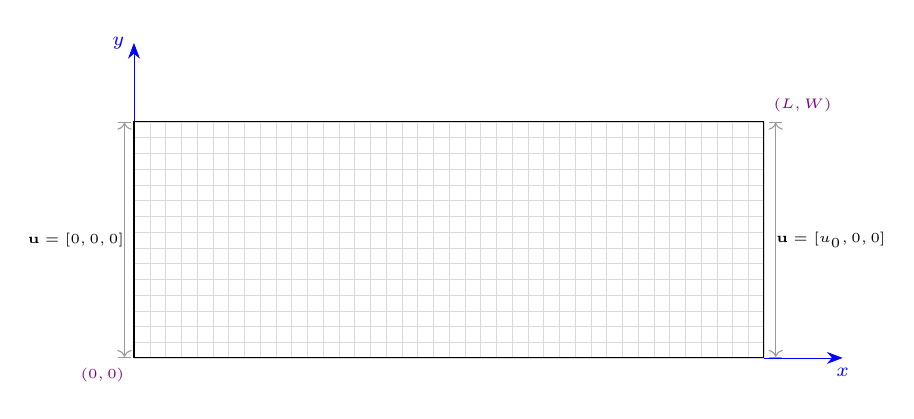
\begin{tikzpicture} [{place/.style={rectangle,draw=blue!50,fill=blue!20,ultra thin,inner sep=0.8mm}},{place2/.style={circle,draw=black!50,ultra thin,inner sep=0.8mm}},{linest/.style={color=gray,ultra thin}}]
	%%coordinates of corners of Beam
	\coordinate (A) at (0.0,0.0);
	\coordinate (B) at (8,0.0);
	\coordinate (D) at ($(A)+(0.0,3.0)$);
	\coordinate (C) at ($(B)+(D)$);
	%%axes
	\draw [{Stealth[length=2mm]}-{Stealth[length=2mm]}, help lines,blue] ($(B)+(1,0)$) -- (A) -- ($(D)+(0,1)$);
	\node [below,color = blue,font=\scriptsize] at ($(B)+(1,0)$) {$x$};
	\node [left,color = blue,font=\scriptsize] at ($(D)+(0,1)$) {$y$};
	%%mesh
	\draw [line width=0.1pt,gray!30,step=2mm](A) grid (C);
	%%Beam	
	\draw [color=black](A)node[font=\tiny, violet,below left]{$(0,0)$} -- (B) -- (C) node[font=\tiny, violet,above right]{$(L,W)$} -- (D) -- cycle;
	%%Concentrate Force Vector
	%\draw [-{Latex[length=2mm]},color=purple, thick] ($(C)+(0.0,1.0)$) -- (C);
	%\node[above,color=purple] at ($(C)+(0.0,1.0)$) {$P$};
	%%B.C
	\draw [|<->|,gray!80]($(B)+(0.15,0.0)$)--($(C)+(0.15,0.0)$) node [fill=white,midway, right, font=\tiny, inner sep=0.05pt, text=black] {$\mathbf{u}=[u_0,0,0]$};
	
	\draw [|<->|,gray!80]($(A)+(-0.12,0.0)$)--($(D)+(-0.12,0.0)$) node [fill=white,midway,left, font=\tiny, inner sep=0.05pt, text=black] {$\mathbf{u}=[0,0,0]$};
	\end{tikzpicture}
\end{document}
	\caption{Geometry, BC and computational domain used for the analysis of linear elasticity.}
	\label{fig_SB}
\end{figure}

For validating our result in this case because of the specific geometry, the deflection of cantilever beam with single fixed support gives a proper estimate. The solution can be retrieve by simple equation as 
\begin{equation}\label{eq1}
	\begin{aligned}
		\delta = \frac{FL^3}{3EI}
	\end{aligned}
\end{equation}
where $F$ is the end load, $I$ denotes the moment of inertia and $E$ is Young's Modulus. In our computational model, we have used Dirichlet BC on $x=0$, and Neumann BC along the line $x=L$, as depicted in Figure \ref{fig_SB}. The domain with Length and width of $L$, $W$ and uniform thickness of $t$. note that the material properties are as follows: Elasticity module and Poisson's ratio are $E$ and $\nu$.
\section{Governing Equations} \label{sec: ge}
The governing equations for the plane elasticity problems discussed above are summarized below, Cauchy momentum equation for a domain $\Omega \subset \mathbb{R}^n$ with boundary $\partial \Omega$ is like:
\begin{equation}\label{eq2}
	\begin{aligned}
		\frac{D \boldsymbol{\upsilon}}{Dt}  &=\frac{1}{\rho} \nabla \cdot \boldsymbol{\sigma} + \mathbf{f} \quad \text{in} \ \Omega\thinspace,\\
		\boldsymbol{\sigma} \cdot \mathbf{n} &= \mathbf{\hat{t}} \quad \text{on} \ \Gamma_N\thinspace,\\
		\mathbf{u}&= \mathbf{\hat{u}}\quad \text{on} \ \Gamma_D\thinspace.
	\end{aligned}
\end{equation}
where $\boldsymbol{\upsilon}$ is the velocity vector field , $t$ is time,
$\frac {D\boldsymbol{\upsilon}}{Dt}$ is the material derivative of $\boldsymbol{\upsilon}$, $\rho$  is the density at a given point, $\boldsymbol {\sigma }$ is the stress tensor, and $\mathbf{f}$ is a vector containing all of the accelerations caused by body forces. So for the expanded form of equations of motion for 2D space we would have
\begin{equation}\label{eq3}
	\begin{aligned}
		\rho \frac{\partial^2 u_x}{\partial t^2}&= \frac{\partial \sigma_{xx}}{\partial x} +  \frac{\partial \sigma_{xy}}{\partial y} + f_x\thinspace,\\
		\rho \frac{\partial^2 u_y}{\partial t^2}&= \frac{\partial \sigma_{xy}}{\partial x} +  \frac{\partial \sigma_{yy}}{\partial y} + f_y\thinspace.
	\end{aligned}
\end{equation}
where $f_x$ and $f_y$ denote the components of the body force vector measured per unit volume along the $x$ and $y$ directions. respectively. here for the sake of simplicity we consider static problem\footnote{Applying time discritization into HiperLife is explained in the transient heat transfer tutorial.}.
\section{Weak Form} \label{sec: wf}
The starting point for the development of the finite element models of Eq. (\ref{eq1}) is their weak forms. The variation formulation of our model problem can be introduced as find $\mathbf{u} \in V$ such that
\begin{equation}\label{eq4}
	\begin{aligned}
		\mathcal{F}(\mathbf{u};v) = 0 \quad \forall v \in \hat{V}\thinspace.
	\end{aligned}
\end{equation}
where
\begin{equation}\label{eq5}
	\begin{aligned}
		\mathcal{F}(\mathbf{u}; v) =\int_{\Omega} v\nabla \cdot \boldsymbol{\sigma} + v \rho \mathbf{f}\mathrm{d}\Omega \thinspace .
	\end{aligned}
\end{equation}
and
\begin{equation}\label{eq6}
	\begin{aligned}
		\hat{V} &= \{v \in H^1(\Omega) : v = 0 \text{ on } \Gamma\}, \\
		V &= \{v \in H^1(\Omega) : v = 0 \text{ on } x=0\}\thinspace.
	\end{aligned}
\end{equation}
where $v$ is a test function, which will be equated, in the our FE model to the interpolation function used for $\mathbf{u}$.

Applying integration by part, and also considering boundary condition, the weak form takes the following form
\begin{equation}\label{eq7}
	\begin{aligned}
		\mathcal{F}(\mathbf{u}; v) &=\int_{\Omega} \nabla \cdot[v\boldsymbol{\sigma}]\mathrm{d}\Omega  - \int_{\Omega} \boldsymbol{\sigma} \nabla v \mathrm{d}\Omega + v \rho \mathbf{f}\mathrm{d}\Omega\\
		 &= \int_{\Gamma} v\boldsymbol{\sigma} \cdot \mathbf{n} \mathrm{d}\Gamma - \int_{\Omega} \boldsymbol{\sigma} \nabla v \mathrm{d}\Omega + \int_{\Omega}v \rho \mathbf{f}\mathrm{d}\Omega\\
		 &=  \int_{\Gamma} v\mathbf{\hat{t}} \mathrm{d}\Gamma - \int_{\Omega} \boldsymbol{\sigma} \nabla v \mathrm{d}\Omega + \int_{\Omega} v \rho \mathbf{f}\mathrm{d}\Omega\thinspace .
	\end{aligned}
\end{equation}
In general, the stress-strain relation for a linear elastic material can be considered as
\begin{equation}\label{eq8}
	\begin{aligned}[b]
		\sigma_{ij} = C_{ijkl} \varepsilon_{kl}
	\end{aligned}
\end{equation}
where $\sigma_{ij}$ and $C_{ijkl}$ are the components of the Cauchy stress tensor and the elasticity tensor ($C_{ijkl} = \lambda\delta_{ij} \delta_{kl} + \mu[\delta_{ik} \delta_{jl} + \delta_{il} \delta_{jk}]$).The  $\boldsymbol{\varepsilon}_{kl}$ are the components of the strain tensor, which by definition is  $\boldsymbol{\varepsilon} = \frac{1}{2}(\nabla \mathbf{u} + \nabla \mathbf{u} ^ T) $, where $\mathbf{u}$ is displacement vector. In simple plane stress case and for isotropic elastic materials the Eq. (\ref{eq8}) takes following format
\begin{equation}\label{eq9}
	\begin{aligned}[b]
		\sigma_{i} &= \mathbf{c}_{ij} \varepsilon_{j}\\
		\begin{Bmatrix}
			\sigma_{xx}\\
			\sigma_{yy}\\
			\sigma_{xy}\\
		\end{Bmatrix}
		&= \begin{bmatrix}
			c_{11} & c_{12} & 0 \\
			c_{12} & c_{22} & 0 \\
			0 & 0 & c_{33} \\
		\end{bmatrix}
		\begin{Bmatrix}
			\varepsilon_{xx}\\
			\varepsilon_{yy}\\
			\varepsilon_{xy}\\
		\end{Bmatrix}
	\end{aligned}
\end{equation}
where $c_{11}=c_{22}=\frac{E}{1-\nu^2}$ and $c_{12}=\nu c_{11}$ and $c_{33} = \frac{1-\nu}{2}c_{11}$.  Considering ($hdA=dV$)  and $\mathbf{u} = \{u_x, u_y\}$ we can rewrite The Eq. (\ref{eq6}) in an explicit form as \cite{reddy2005introduction}
\begin{equation}\label{eq10}
	\begin{aligned}[b]
		&\int_{\Omega} h \left[\frac{\partial v}{\partial x}\left(c_{11}\frac{\partial u_x}{\partial x} + c_{12}\frac{\partial u_y}{\partial y} \right) + c_{33}\frac{\partial v}{\partial y}\left(\frac{\partial u_x}{\partial y} + \frac{\partial u_y}{\partial x} \right)\right]  \ dA = 	\int_{\Omega} h v f_x \ dA + \int_{\Gamma} h v t_x \ dS \thinspace,\\
		&\int_{\Omega} h \left[c_{33}\frac{\partial v}{\partial x}\left(\frac{\partial u_x}{\partial y} + \frac{\partial u_y}{\partial x} \right) + \frac{\partial v}{\partial y}\left(c_{12}\frac{\partial u_x}{\partial x} + c_{22}\frac{\partial u_y}{\partial y} \right)\right]  \ dA = 	\int_{\Omega} h v f_y \ dA +\int_{\Gamma} h v t_y \ dS\thinspace.
	\end{aligned}
\end{equation}
\section{Finite Element Model} \label{sec: fem}
Since we are developing the Ritz-Galerkin finite element model, the choice of the weight functions is restricted to the spaces of approximation functions used for the solution field. Suppose that the displacement approximated by expansions of the form
\begin{equation}\label{eq11}
	\begin{aligned}
		u(x,y)= \sum_{m=1}^{M} \phi_m(x,y) \mathbf{u}^m= \boldsymbol{\Phi}^T\mathbf{u} \thinspace,
	\end{aligned}
\end{equation}
By substitution of Eq. (\ref{eq11}) to Eq. (\ref{eq10})and writing the resulting algebraic equations in matrix form, we obtain
\begin{equation}\label{eq12}
	\begin{aligned}[b]
		\begin{bmatrix}
			[K^{11}] & [K^{12}]\\
			[K^{21}] & [K^{22}]\\
		\end{bmatrix}
		\begin{Bmatrix}
			\{u_x\}\\
			\{u_y\}\\
		\end{Bmatrix}
		= \begin{Bmatrix}
			\{F^1\}\\
			\{F^2\}\\
		\end{Bmatrix}
	\end{aligned}
\end{equation}
where
\begin{equation}\label{eq13}
	\begin{aligned}[b]
		K^{11}_{ij} &= \int_{\Omega^e} h \left[c_{11}\frac{\partial \phi_i}{\partial x}\frac{\partial \phi_j}{\partial x} +c_{33}\frac{\partial \phi_i}{\partial y}\frac{\partial \phi_j}{\partial y}\right]  \ dxdy\\
		K^{22}_{ij} &= \int_{\Omega^e} h \left[c_{33}\frac{\partial \phi_i}{\partial x}\frac{\partial \phi_j}{\partial x} +c_{22}\frac{\partial \phi_i}{\partial y}\frac{\partial \phi_j}{\partial y}\right]  \ dxdy\\
		K^{12}_{ij} &= K^{21}_{ji} = \int_{\Omega^e} h \left[c_{12}\frac{\partial \phi_i}{\partial x}\frac{\partial \phi_j}{\partial y} +c_{33}\frac{\partial \phi_i}{\partial y}\frac{\partial \phi_j}{\partial x}\right]  \ dxdy\\
		F^{1}_{i} &= \int_{\Omega^e} h \phi_i f_x \ dxdy +\int_{\Gamma^e} h \phi_i t_x \ ds\\
		F^{2}_{i} &= \int_{\Omega^e} h \phi_i f_y \ dxdy +\int_{\Gamma^e} h \phi_i t_y \ ds\\
	\end{aligned}
\end{equation}
The elemental representation of the vector and matrix required for implementation in the Hiperlife would be
like
\begin{equation}\label{eq13}
	\begin{aligned}[b]
		Ak(i,0,j,0)&=K^{11}_{ij} \quad , \quad Ak(i,0,j,1)=K^{12}_{ij}\\
		Ak(i,1,j,0)&=K^{21}_{ij}\quad , \quad Ak(i,1,j,1)=K^{22}_{ij} \\
		Bk(i,0)&=F^{1}_{i} \quad , \quad 		Bk(i,1)=F^{2}_{i}\\
	\end{aligned}
\end{equation}
\section{Choice of Elements} \label{sec: coe}
Thus, for this simple problem every Lagrange and serendipity family of interpolation functions are admissible for the interpolation of the temperature field, our choice is would be linear quadrilateral element.Linear  Quadrilateral Elements is the simplest quadrilateral element consists of four nodes. The associated interpolation functions for geometry and field variables are bilinear.
\begin{equation}\label{eq11}
	\begin{aligned}[b]
		\boldsymbol{\Phi}_{I}(\xi, \eta) = \frac{1}{4}(1+\xi_I\xi)(1+\eta_I\eta) \quad (I \ \text{from} \ 1 \ \text{to} \ 4)
	\end{aligned}
\end{equation}
where $\xi_{I}$ and $\eta_{I}$ are the corner coordinates at element $T$ in domain of $\Omega_{T} \in (-1,1)^2$. As it shown in Figure \ref{fig_el} we are using $2 \times 2$ Gauss–Legendre quadrature integration.
\begin{figure}[htbp]
	\centering
	\documentclass[preprint,12pt,a4]{standalone}
\usepackage{geometry}   % my added package "geometry"
\geometry{letterpaper,tmargin=1in,bmargin=1in,lmargin=2.5cm,rmargin=2.5cm}
\usepackage{tikz}
\usetikzlibrary{calc,patterns,arrows.meta,shapes.arrows,intersections,positioning}
\usetikzlibrary{decorations.pathmorphing,backgrounds,fit,petri}
\usepackage{standalone}
%
\begin{document}
	\begin{tikzpicture} [{place/.style={rectangle,draw=blue!50,fill=blue!20,ultra thin,inner sep=0.8mm}},{place2/.style={circle,draw=black!50,ultra thin,inner sep=0.8mm}},{linest/.style={color=gray,ultra thin}}]
		%axes
		\draw [{Stealth[length=2mm]}-{Stealth[length=2mm]}, help lines,blue] (5.0,0)node[above,font=\scriptsize]{$\xi$} -- (0.0,0.0) -- (0.0,5.0)node[right,font=\scriptsize] {$\eta$};
		%%corner nodes
		\node at (0.0,0.0) [place,fill=violet!60] (1) {};
		\node at (4.0,0.0) [place,fill=violet!60] (2) {};
		\node at (4.0,4.0) [place,fill=violet!60] (3) {};
		\node at (0.0,4.0) [place,fill=violet!60] (4) {};
		%% integration points
	    \node at (1.0,1.0) [place2,fill=gray!60] (5) {};
		\node at (3.0,1.0) [place2,fill=gray!60] (6) {};
		\node at (1.0,3.0) [place2,fill=gray!60] (7) {};
		\node at (3.0,3.0) [place2,fill=gray!60] (8) {};
		%%element border
		\draw [-,black] (1) -- (2) -- (3) -- (4) --(1);
		%%middle nodes
		\node at (5.6,2.5) [right,font=\scriptsize]{$\mathrm{Element \ nodes}$};
		\node at (5.5,2.5) [place,fill=violet!60] (4) {};
		\node at (5.6,2.2) [right,font=\scriptsize]{$\mathrm{integration \ points}$};
		\node at (5.5,2.2) [place2,fill=gray!60] (4) {};
		
	\end{tikzpicture}
\end{document}
	\caption{Linear quadrilateral element used for finite element model.}
	\label{fig_el}
\end{figure}

We also choose a uniform mesh of $100 \times 12$ to model our domain $[0,2] \times[0,0.12]$.
\section{Implementation} \label{sec: im}
In this section, we present the implementation of our solution in the Hiperlife. The program is divided into three separate files, main part which we create our problem by the Hiperlife headers, auxiliary header where we introduce parameters and declare defined functions, and at last auxiliary file, where we define some functions which provide required matrices like Jacobian and Hessian.
\subsubsection{PlaneStress2D.cpp} \label{sec: m.cpp}
\nolinenumbers
\begin{lstlisting}
/*
*******************************************************************************
linear elasticity 2-D Plane stress
*******************************************************************************
*/

// cpp headers
#include <iostream>
#include <fstream>
#include <time.h>

// hiperlife headers
#include "hl_Core.h"
#include "hl_ParamStructure.h"
#include "hl_Parser.h"
#include "hl_TypeDefs.h"
#include "hl_MeshLoader.h"
#include "hl_StructMeshGenerator.h"
#include "hl_DistributedMesh.h"
#include "hl_FillStructure.h"
#include "hl_DOFsHandler.h"
#include "hl_HiPerProblem.h"
#include "hl_SurfLagrParam.h"
#include "hl_LinearSolver_Iterative_AztecOO.h"
#include "hl_LinearSolver_Direct_MUMPS.h"
#include "hl_GlobalBasisFunctions.h"

// Header to auxiliary functions
#include "Aux2D.h"

// ----------------------- MAIN FUNCTION ------------------------------//
int main(int argc, char** argv)
{
	using namespace std;
	using namespace hiperlife;
	using hiperlife::Tensor::tensor;
	
	//---------------------INITIALIZATION------------------------------//
	hiperlife::Init(argc, argv);
	
	//---------------------------STRUCT--------------------------------//
	SmartPtr<ParamStructure> paramStr = CreateParamStructure<PlaneStressParams>();
	const double traction = paramStr->getRealParameter(PlaneStressParams::traction);
	//------------------------MESH CREATION----------------------------//
	SmartPtr<StructMeshGenerator> structMesh = Create<StructMeshGenerator>();
	
	structMesh->setNDim(3);
	structMesh->setBasisFuncType(BasisFuncType::Lagrangian);
	structMesh->setBasisFuncOrder(1);
	structMesh->setElemType(ElemType::Square);
	structMesh->genRectangle(100, 12, 2.0, 0.12);
	SmartPtr<DistributedMesh> disMesh = Create<DistributedMesh>();
	disMesh->setMesh(structMesh);
	disMesh->setBalanceMesh(true);
	disMesh->setElementLocatorEngine(ElementLocatorEngine::BoundingVolumeHierarchy);
	disMesh->Update();
	//----------------------DOFsHANDLER CREATION-----------------------//
	// ----------------------- Displacement--------------------------- //
	SmartPtr<DOFsHandler> dofHand = Create<DOFsHandler>(disMesh);
	dofHand->setNameTag("dofHand");
	dofHand->setNumDOFs(2);
	dofHand->setDOFs({"u","v"});
	dofHand->Update();
	//-------------------------- B.C ----------------------------------//
	//------------------ Dirichlet on the left side -------------------//
	dofHand->setBoundaryCondition(0, MAxis::Xmin, 0.0);
	dofHand->setBoundaryCondition(1, MAxis::Xmin, 0.0);
	
	//dofHand->setBoundaryCondition(1, MAxis::Xmax, 0.01);
	
	dofHand->UpdateGhosts();
	//---------------------------------------------------------------- //
	//--------------------HIPERPROBLEM CREATION------------------------//
	// -------------------------- Displacement ----------------------- //
	SmartPtr<HiPerProblem> hiperProbl = Create<HiPerProblem>();
	
	hiperProbl->setParameterStructure(paramStr);
	hiperProbl->setDOFsHandlers({dofHand});
	
	hiperProbl->setIntegration("Integ", {"dofHand"});
	hiperProbl->setCubatureGauss("Integ", 4);
	hiperProbl->setElementFillings("Integ", ElementFilling);
	
	// Nuemann boundary condition: Set integration on the border
	hiperProbl->setIntegration("BorderInteg", {"dofHand"});
	hiperProbl->setCubatureBorderGauss("BorderInteg",1,{MAxis::Xmax});
	hiperProbl->setElementFillings("BorderInteg", nullptr, nullptr, RHS_Border);
	
	hiperProbl->Update();
	
	//-----------------------SOLVER CREATION---------------------------//
	// ---------------------- Displacement --------------------------- //
	SmartPtr<MUMPSDirectLinearSolver> solver = Create<MUMPSDirectLinearSolver>();
	solver->setHiPerProblem(hiperProbl);
	solver->setVerbosity(MUMPSDirectLinearSolver::Verbosity::Extreme);
	solver->setDefaultParameters();
	solver->Update();
	
	solver->solve();
	hiperProbl->UpdateSolution();
	
	dofHand->printFileLegacyVtk("PlaneStress2D", true);
	
	hiperlife::Finalize();
	return 0;
}

\end{lstlisting}
\subsubsection{Aux2D.h} \label{sec: a.h}
\begin{lstlisting}
#ifndef AUXFLUID_H
#define AUXFLUID_H


#include <iostream>
#include <fstream>
#include <time.h>

// Hiperlife headers
#include "hl_Core.h"
#include "hl_ParamStructure.h"
#include "hl_Parser.h"
#include "hl_TypeDefs.h"
#include "hl_MeshLoader.h"
#include "hl_StructMeshGenerator.h"
#include "hl_DistributedMesh.h"
#include "hl_FillStructure.h"
#include "hl_DOFsHandler.h"
#include "hl_HiPerProblem.h"
#include "hl_SurfLagrParam.h"
#include "hl_LinearSolver_Iterative_AztecOO.h"
#include "hl_GlobalBasisFunctions.h"

using namespace std;
using namespace hiperlife;
using hiperlife::Tensor::tensor;

struct PlaneStressParams
{
	enum RealParameters
	{
		thickness,
		E,
		nu,
		traction
	};
	
	HL_PARAMETER_LIST DefaultValues
	{
		{"thickness", 0.02},
		{"E", 200000000000.0},
		{"nu", 0.3},
		{"traction", 2000000000.0},
	};
};

void ElementFilling(hiperlife::FillStructure& fillStr);
void RHS_Border(hiperlife::FillStructure& fillStr);


#endif

\end{lstlisting}
\subsubsection{Aux2D.cpp} \label{sec: a.cpp}
\begin{lstlisting}
// Header to auxiliary functions
#include "Aux2D.h"

#include <iostream>
#include <fstream>
#include <time.h>

// Hiperlife headers
#include "hl_Core.h"
#include "hl_ParamStructure.h"
#include "hl_Parser.h"
#include "hl_TypeDefs.h"
#include "hl_MeshLoader.h"
#include "hl_StructMeshGenerator.h"
#include "hl_DistributedMesh.h"
#include "hl_FillStructure.h"
#include "hl_DOFsHandler.h"
#include "hl_HiPerProblem.h"
#include "hl_SurfLagrParam.h"
#include "hl_LinearSolver_Iterative_AztecOO.h"
#include "hl_GlobalBasisFunctions.h"

// --------------------------------------------------------------------//
// -------------------------- FUNCTIONS -------------------------------//
// --------------------------------------------------------------------//

void ElementFilling(hiperlife::FillStructure& fillStr)
{
	using namespace std;
	using namespace hiperlife;
	using hiperlife::Tensor::tensor;
	
	
	const long double E = fillStr.getRealParameter(PlaneStressParams::E);
	const double nu = fillStr.getRealParameter(PlaneStressParams::nu);
	const double thickness = fillStr.getRealParameter(PlaneStressParams::thickness);
	
	
	//--------------------------Velocity-related----------------------//
	// Dimensions
	SubFillStructure& subFill = fillStr["dofHand"];
	int eNN  = subFill.eNN;
	int pDim = subFill.pDim;
	int numDOFs = subFill.numDOFs; // numDOFs = 2
	
	// Shape functions and derivatives at Gauss points
	tensor<double,1,false>  bf(subFill.nborBFs(),eNN);
	tensor<double,2> Dbf_g(eNN, pDim);
	double jac;
	GlobalBasisFunctions::gradients(Dbf_g, jac, subFill);
	
	ttl:: wrapper<double,4> Ak(fillStr.Ak(0, 0).data(),eNN, numDOFs, eNN, numDOFs);
	ttl:: wrapper<double,2> Bk(fillStr.Bk(0).data(), eNN, numDOFs);
	
	
	// Elasticity Tensor
	ttl::tensor<long double,2> C{{E/(1.0 -nu*nu), E*nu/(1.0-nu*nu), 0.0},
		{E*nu/(1.0-nu*nu), E/(1.0-nu*nu), 0.0},{0.0, 0.0, E/(1.0+nu)}};
	ttl::tensor<double,1> F{0.0,0.0};
	
	for (int i=0;i < eNN;i++)
	{
		for (int j=0;j < eNN;j++)
		{
			Ak(i,0,j,0) += thickness * jac * 
			(C(0,0)*Dbf_g(i,0)*Dbf_g(j,0) + C(2,2)*Dbf_g(i,1)*Dbf_g(j,1));
			Ak(i,0,j,1) += thickness * jac * 
			(C(0,1)*Dbf_g(i,0)*Dbf_g(j,1) + C(2,2)*Dbf_g(i,1)*Dbf_g(j,0));
			Ak(i,1,j,0) += thickness * jac * 
			(C(0,1)*Dbf_g(i,1)*Dbf_g(j,0) + C(2,2)*Dbf_g(i,0)*Dbf_g(j,1));
			Ak(i,1,j,1) += thickness * jac * 
			(C(1,1)*Dbf_g(i,0)*Dbf_g(j,0) + C(2,2)*Dbf_g(i,1)*Dbf_g(j,1));
		}
		Bk(i,0) += thickness * jac * bf(i) * F(0);
		Bk(i,1) += thickness * jac * bf(i) * F(1);
	}
	
}
void RHS_Border(hiperlife::FillStructure& fillStr)
{
	using namespace std;
	using namespace hiperlife;
	using hiperlife::Tensor::tensor;
	
	const double thickness = fillStr.getRealParameter(PlaneStressParams::thickness);
	const double traction = fillStr.getRealParameter(PlaneStressParams::traction);
	// Variables
	SubFillStructure& subFill = fillStr["dofHand"];
	int DOF  = subFill.numDOFs;
	int eNN  = subFill.eNN;
	int nDim = subFill.nDim;
	vector<double>& nborCoords = subFill.nborCoords;
	double *bf  = subFill.nborBFs();
	double *dbf_l = subFill.nborBFsGrads();
	
	ttl:: wrapper<double,2> Bk(fillStr.Bk(0).data(), eNN, DOF);
	
	double Ip[4], xu[3], xv[3];
	SurfLagrParam::MetricTensor(Ip, xu, xv, eNN, nborCoords.data(), dbf_l);
	
	// Compute jacobian
	auto bTangentRef = subFill.tangentsBoundaryRef();
	double bTangent[3]={};
	for (int n = 0; n < nDim; n++)
	bTangent[n] = bTangentRef[0] * xu[n] + bTangentRef[1]*xv[n];
	double jac = Math::Norm3D(bTangent);
	
	// Fill RHS
	for (int i = 0; i < eNN; i++)
	fillStr.Bk(0)[i*DOF+1] += jac*bf[i]*traction * thickness;
}
\end{lstlisting}
\section{Results} \label{sec: rst}
In this section we present our solution. Figures \ref{fig_Rs1} and \ref{fig_Rs1} show the displacement contour in deformed configuration.

\begin{figure}[htbp]
	\centering
		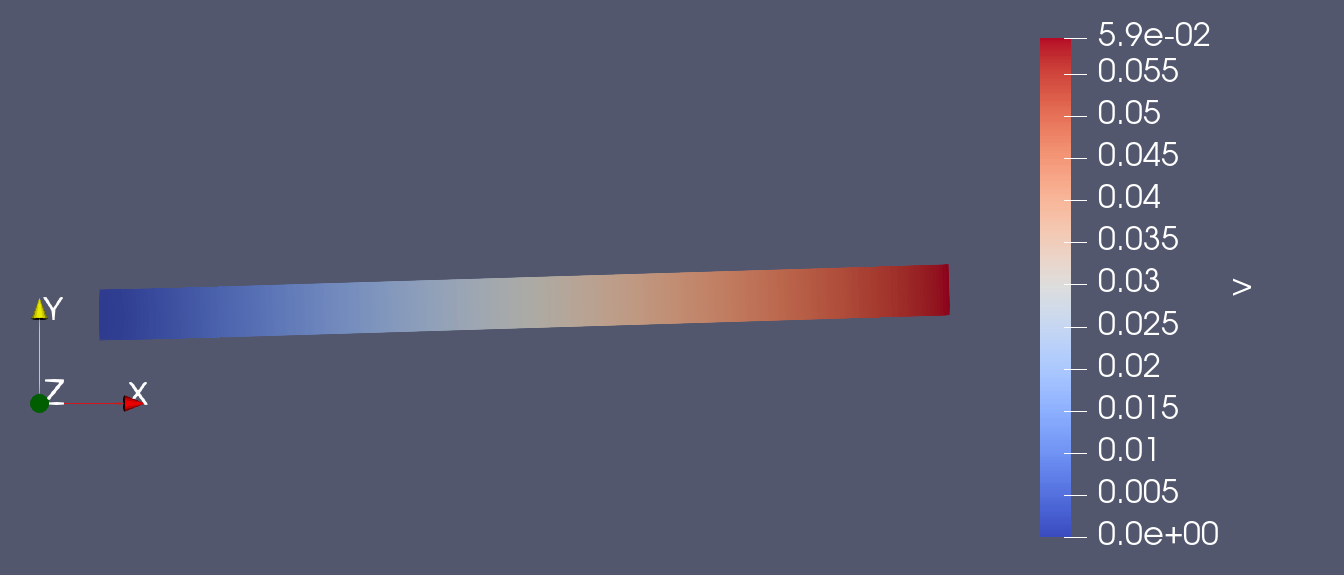
\includegraphics[width=\textwidth]{Figures/result1.png}
		\caption{Displacement in y-direction.}
		\label{fig_Rs1}
	\hfill
		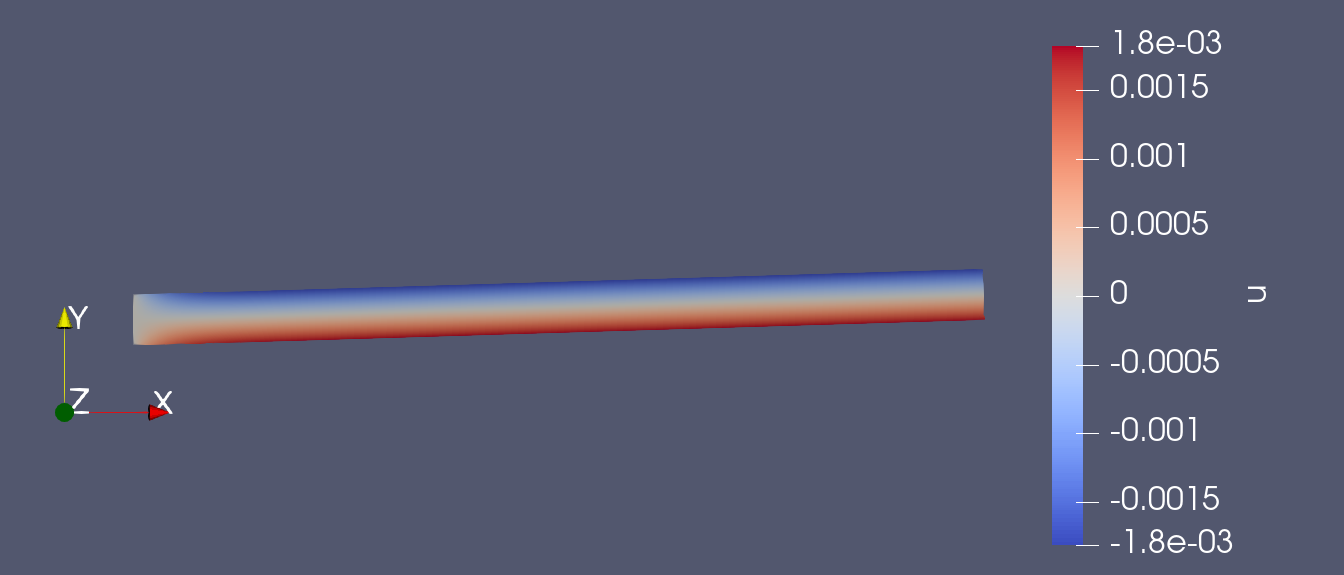
\includegraphics[width=\textwidth]{Figures/result2.png}
		\caption{Displacement in x-direction.}
	\label{fig_Rs2}
\end{figure}

\bibliographystyle{unsrt}
\bibliography{ref}
\end{document}
